\documentclass[tikz,border=3.14mm]{standalone}
\usepackage{pgfplots}
\pgfplotsset{compat=1.18}

\begin{document}
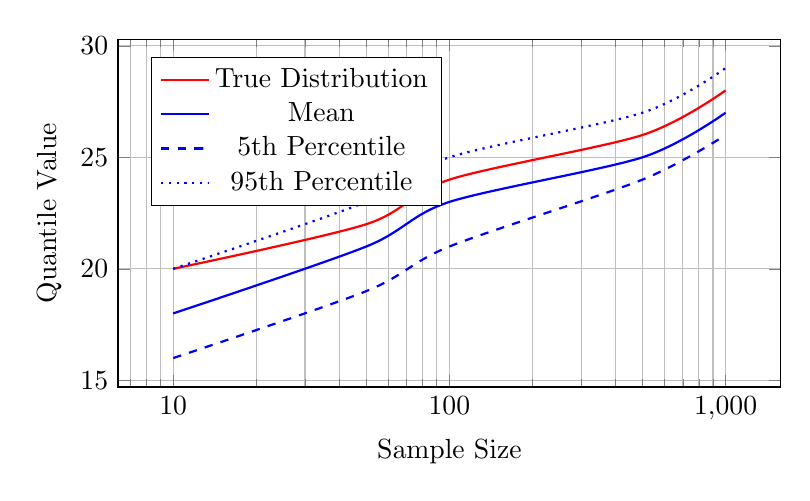
\begin{tikzpicture}
\begin{axis}[
    width=10cm,
    height=6cm,
    xlabel={Sample Size},
    ylabel={Quantile Value},
    xmode=log,
    log ticks with fixed point,
    grid=both,
    legend style={at={(0.05,0.95)}, anchor=north west},
    smooth
]

% True distribution (red line)
\addplot[color=red, thick, mark=none] 
    coordinates {(10, 20) (50, 22) (100, 24) (500, 26) (1000, 28)};
\addlegendentry{True Distribution}

% Estimator mean (solid blue)
\addplot[color=blue, thick, mark=none]
    coordinates {(10, 18) (50, 21) (100, 23) (500, 25) (1000, 27)};
\addlegendentry{Mean}

% 5th percentile (dashed blue)
\addplot[color=blue, dashed, thick, mark=none]
    coordinates {(10, 16) (50, 19) (100, 21) (500, 24) (1000, 26)};
\addlegendentry{5th Percentile}

% 95th percentile (dotted blue)
\addplot[color=blue, dotted, thick, mark=none]
    coordinates {(10, 20) (50, 23) (100, 25) (500, 27) (1000, 29)};
\addlegendentry{95th Percentile}

\end{axis}
\end{tikzpicture}
\end{document}